\section{Interactive Plotting}

\begin{frame}[fragile]
  \frametitle{First Plot}
  \begin{itemize}
  \item Start IPython with \texttt{-pylab}
  \end{itemize}
  \begin{lstlisting}
    $ ipython -pylab
  \end{lstlisting}  % $
  \begin{lstlisting}
   In[]: p = linspace(-pi,pi,100) 
   In[]: plot(p, cos(p))
  \end{lstlisting}
\end{frame}


\begin{frame}[fragile]
  \frametitle{\texttt{linspace}}
  \begin{itemize}
  \item \texttt{p} has a hundred points in the range -pi to pi
    \begin{lstlisting}
     In[]: print p[0], p[-1], len(p)
    \end{lstlisting}
  \item Look at the doc-string of \texttt{linspace} for more details
    \begin{lstlisting}
     In[]: linspace?
    \end{lstlisting}
  \end{itemize}
  \begin{itemize}
  \item \texttt{plot} simply plots the two arguments with default
    properties 
  \end{itemize}
\end{frame}

\section{Embellishing Plots}

\begin{frame}[fragile]
  \frametitle{Plot color and thickness}
  \begin{lstlisting}
   In[]: clf()
   In[]: plot(p, sin(p), 'r')
  \end{lstlisting}
  \begin{itemize}
  \item Gives a sine curve in Red. 
  \end{itemize}
  \begin{lstlisting}
   In[]: plot(p, cos(p), linewidth=2)
  \end{lstlisting}
  \begin{itemize}
  \item Sets line thickness to 2
  \end{itemize}
  \begin{lstlisting}
   In[]: clf()
   In[]: plot(p, sin(p), '.')
  \end{lstlisting}
  \begin{itemize}
  \item Produces a plot with only points
  \end{itemize}
  \begin{lstlisting}
   In[]: plot?
  \end{lstlisting}
\end{frame}

\begin{frame}[fragile]
  \frametitle{\texttt{title}}
  \begin{lstlisting}
   In[]: x = linspace(-2, 4, 50)
   In[]: plot(x, -x*x + 4*x - 5, 'r', 
         linewidth=2)
   In[]: title("Parabolic function -x^2+4x-5")
  \end{lstlisting}
  \begin{itemize}
  \item We can set title using \LaTeX~ 
  \end{itemize}
  \begin{lstlisting}
   In[]: title("Parabolic function $-x^2+4x-5$")
  \end{lstlisting} 
\end{frame}

\begin{frame}[fragile]
  \frametitle{Axes labels}
  \begin{lstlisting}
   In[]: xlabel("x")
   In[]: ylabel("f(x)")
  \end{lstlisting}
  \begin{itemize}
  \item We could, if required use \LaTeX~ 
  \end{itemize}
\end{frame}

\begin{frame}[fragile]
  \frametitle{Annotate}
  \begin{lstlisting}
   In[]: annotate("local maxima", xy=(2, -1))
  \end{lstlisting}
  \begin{itemize}
  \item First argument is the annotation text
  \item The argument to \texttt{xy} is a tuple that gives the location
    of the text. 
  \end{itemize}
\end{frame}

\begin{frame}[fragile]
  \frametitle{Limits of Plot area}
  \begin{lstlisting}
   In[]: xlim()
   In[]: ylim()
  \end{lstlisting}
  \begin{itemize}
  \item With no arguments, \texttt{xlim} \& \texttt{ylim} get the
    current limits
  \item New limits are set, when arguments are passed to them
  \end{itemize}
  \begin{lstlisting}
   In[]: xlim(-4, 5)
  \end{lstlisting}
  \begin{lstlisting}
   In[]: ylim(-15, 2)
  \end{lstlisting}
\end{frame}

\begin{frame}
\frametitle{Plot}
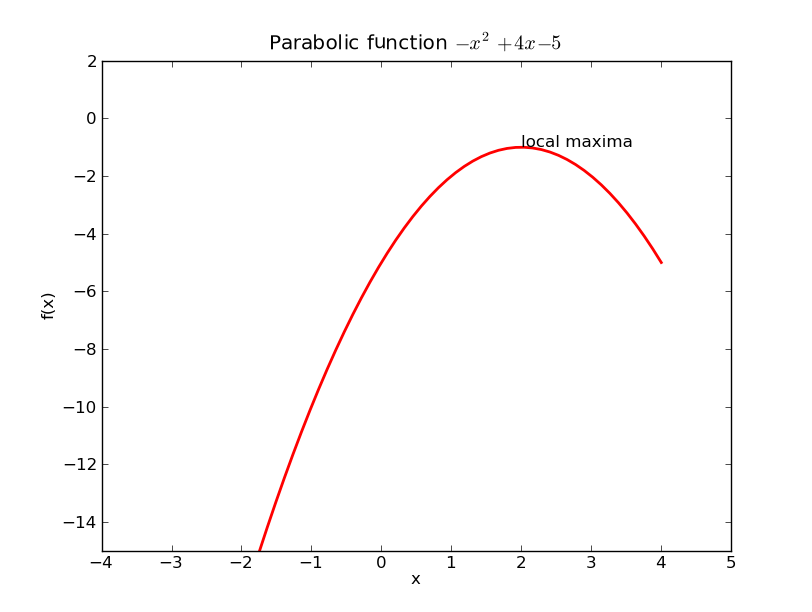
\includegraphics[scale=0.45]{../advanced_python/images/plot.png}\\
\end{frame}



\section{Saving to Scripts}

\begin{frame}[fragile]
  \frametitle{Command history}
  \begin{itemize}
  \item To see the history of commands, we typed
    \begin{lstlisting}
     In[]: %hist
    \end{lstlisting}
  \item All commands, valid or invalid, appear in the history
  \item \texttt{\%hist} is a magic command, available only in IPython
  \end{itemize}
  \begin{lstlisting}
   In[]: %hist 5
    # last 5 commands
  \end{lstlisting}
  \begin{lstlisting}
   In[]: %hist 5 10
    # commands between 5 and 10
  \end{lstlisting}
\end{frame}

\begin{frame}[fragile]
  \frametitle{Saving to a script}
  \begin{itemize}
  \item We wish to save commands for reproducing the parabola
  \item Look at the history and identify the commands that will
    reproduce the parabolic function along with all embellishment
  \item \texttt{\%save} magic command to save the commands to a file
  \end{itemize}
  \begin{lstlisting}
   In[]: %save plot_script.py 1 3-6 8
  \end{lstlisting}
  \begin{itemize}
  \item File name must have a \texttt{.py} extension
  \end{itemize}
\end{frame}

\begin{frame}[fragile]
  \frametitle{Running the script}
  \begin{lstlisting}
   In[]: %run -i plot_script.py
  \end{lstlisting}
  \begin{itemize}
  \item There were no errors in the plot, but we don't see it!
  \item Running the script means, we are not in interactive mode
  \item We need to explicitly ask for the image to be shown
  \end{itemize}
  \begin{lstlisting}
   In[]: show()
  \end{lstlisting}
  \begin{itemize}
  \item \texttt{-i} asks the interpreter to check for names,
    unavailable in the script, in the interpreter
  \item \texttt{sin}, \texttt{plot}, etc. are taken from the
    interpreter
  \end{itemize}
\end{frame}

\section{Saving Plots}

\begin{frame}[fragile]
  \frametitle{\texttt{savefig}}
  \begin{lstlisting}
   In[]: x = linspace(-3*pi,3*pi,100)
   In[]: plot(x,sin(x))
   In[]: savefig('sine.png')
  \end{lstlisting}
  \begin{itemize}
  \item \texttt{savefig} takes one argument
  \item The file-type is decided based on the extension
  \item \texttt{savefig} can save as png, pdf, ps, eps, svg
  \end{itemize}
\end{frame}

\section{Multiple Plots}

\begin{frame}[fragile]
  \frametitle{Overlaid plots}
  \begin{lstlisting}
   In[]: x = linspace(0, 50, 10)
   In[]: plot(x, sin(x))
  \end{lstlisting}
  \begin{itemize}
  \item The curve isn't as smooth as we expected
  \item We chose too few points in the interval
  \end{itemize}
  \begin{lstlisting}
   In[]: y = linspace(0, 50, 500)
   In[]: plot(y, sin(y))
  \end{lstlisting}
  \begin{itemize}
  \item The plots are overlaid
  \item It is the default behaviour of \texttt{pylab}
  \end{itemize}
\end{frame}

\begin{frame}[fragile]
  \frametitle{Legend}
  \begin{lstlisting}
   In[]: legend(['sine-10 points',
          'sine-500 points'])
  \end{lstlisting}
  \begin{itemize}
  \item Placed in the location, \texttt{pylab} thinks is `best'
  \item \texttt{loc} parameter allows to change the location
  \end{itemize}
  \begin{lstlisting}
   In[]: legend(['sine-10 points',
         'sine-500 points'], 
            loc='center')
  \end{lstlisting}
\end{frame}

\begin{frame}
\frametitle{Overlaid Plots}
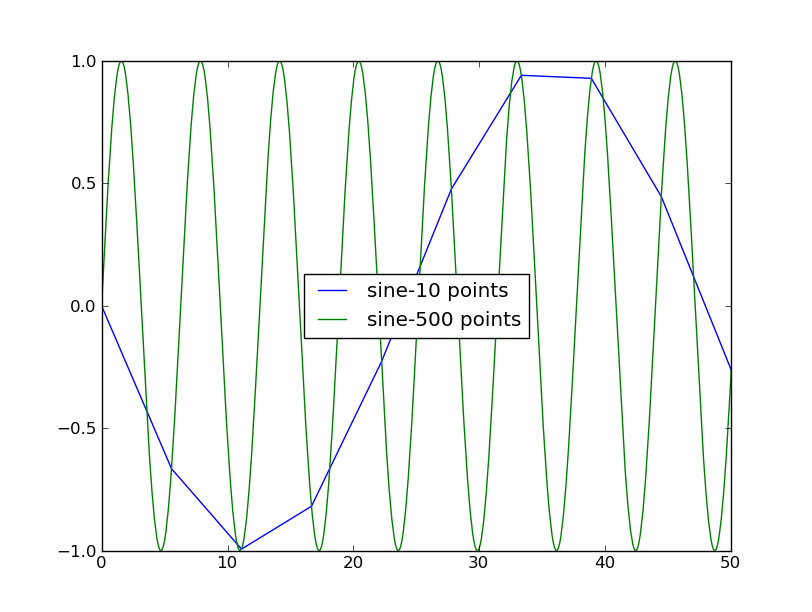
\includegraphics[scale=0.45]{../advanced_python/images/overlaid.png}\\
\end{frame}



\begin{frame}[fragile]
  \frametitle{Plotting in separate figures}
  \begin{lstlisting}
   In[]: clf()
   In[]: x = linspace(0, 50, 500)
   In[]: figure(1)
   In[]: plot(x, sin(x), 'b')
   In[]: figure(2)
   In[]: plot(x, cos(x), 'g')
  \end{lstlisting}
  \begin{itemize}
  \item \texttt{figure} command allows us to have plots separately
  \item It is also used to switch context between the plots
  \end{itemize}
  \begin{lstlisting}
   In[]: savefig('cosine.png')
   In[]: figure(1)
   In[]: title('sin(y)')
   In[]: savefig('sine.png')
   In[]: close()
   In[]: close()
  \end{lstlisting}
  \begin{itemize}
  \item \texttt{close('all')} closes all the figures
  \end{itemize}
\end{frame}

\begin{frame}[fragile]
  \frametitle{Subplots}
  \begin{lstlisting}
   In[]: subplot(2, 1, 1)
  \end{lstlisting}
  \begin{itemize}
  \item number of rows
  \item number of columns
  \item plot number, in serial order, to access or create
  \end{itemize}
  \begin{lstlisting}
   In[]: subplot(2, 1, 2)
   In[]: x = linspace(0, 50, 500)
   In[]: plot(x, cos(x))

   In[]: subplot(2, 1, 1)
   In[]: y = linspace(0, 5, 100)
   In[]: plot(y, y ** 2)
  \end{lstlisting}
\end{frame}

\begin{frame}
\frametitle{Subplots}
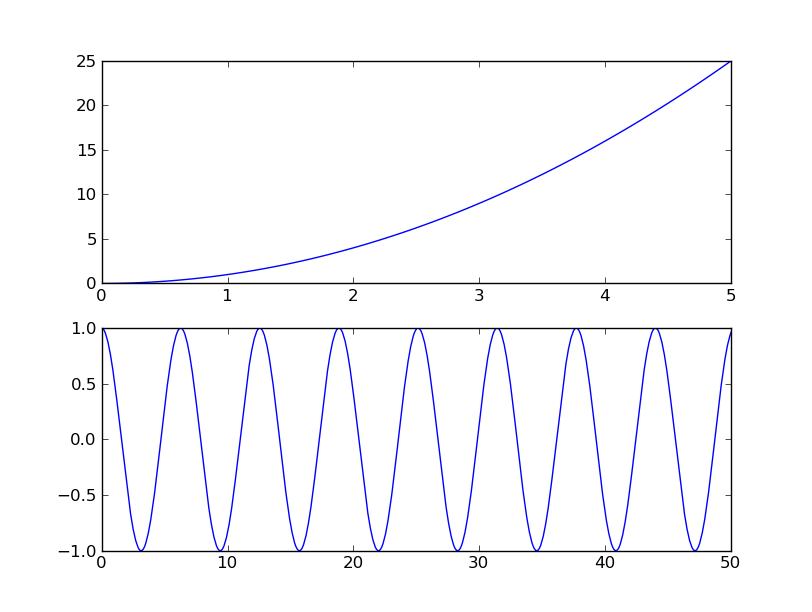
\includegraphics[scale=0.45]{../advanced_python/images/subplot.png}\\
\end{frame}



\section{Plotting Data}

\begin{frame}[fragile]
  \frametitle{Loading data}
  \begin{itemize}
  \item \texttt{primes.txt} contains a list of primes listed
    column-wise
  \item We read the data using \texttt{loadtxt} 
  \end{itemize}
  \begin{lstlisting}
  In[]: primes = loadtxt('primes.txt')
  In[]: print primes
  \end{lstlisting}
  \begin{itemize}
  \item \texttt{primes} is a sequence of floats
  \end{itemize}
\end{frame}

\begin{frame}[fragile]
  \frametitle{Reading two column data}
  \begin{itemize}
  \item \texttt{pendulum.txt} has two columns of data
  \item Length of pendulum in the first column 
  \item Corresponding time period in second column
  \item \texttt{loadtxt} requires both columns to be of same length
  \end{itemize}
  \begin{lstlisting}
   In[]: pend = loadtxt('pendulum.txt')
   In[]: print pend
  \end{lstlisting}
  \begin{itemize}
  \item \texttt{pend} is not a simple sequence like \texttt{primes}
  \end{itemize}
\end{frame}

\begin{frame}[fragile]
  \frametitle{Unpacking with \texttt{loadtxt}}
  \begin{lstlisting}
   In[]: L, T = loadtxt('pendulum.txt',
                 unpack=True)
   In[]: print L
   In[]: print T
  \end{lstlisting}
  \begin{itemize}
  \item We wish to plot L vs. $T^2$
  \item \texttt{square} function gives us the squares
  \item (We could instead iterate over T and calculate)
  \end{itemize}
  \begin{lstlisting}
   In[]: Tsq = square(T)

   In[]: plot(L, Tsq, '.')
  \end{lstlisting}
\end{frame}

\begin{frame}[fragile]
  \frametitle{\texttt{errorbar}}
  \begin{itemize}
  \item Experimental data always has errors
  \item \texttt{pendulum\_error.txt} contains errors in L and T
  \item Read the values and make an error bar plot
  \end{itemize}
  \begin{lstlisting}
  In[]:  L, T, L_err, T_err = \
         loadtxt('pendulum_error.txt',
         unpack=True)
  In[]:  Tsq = square(T)

  In[]:  errorbar(L, Tsq , xerr=L_err, 
         yerr=T_err, fmt='b.')
  \end{lstlisting}
\end{frame}

\begin{frame}
\frametitle{Errorbar}
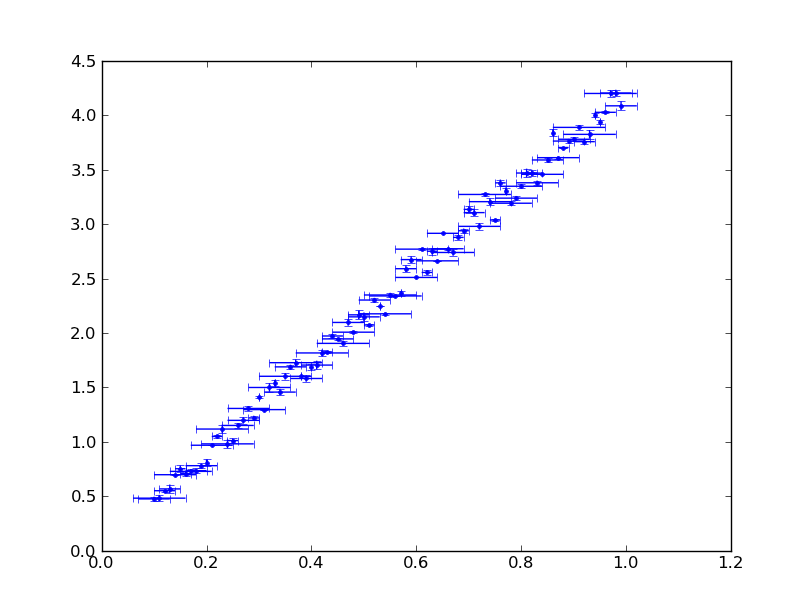
\includegraphics[scale=0.45]{../advanced_python/images/L-Tsq.png}\\
\end{frame}

\section{Other kinds of Plots}

\begin{frame}[fragile]
  \frametitle{Scatter Plot}
  \begin{itemize}
  \item The data is displayed as a collection of points
  \item Value of one variable determines position along x-axis
  \item Value of other variable determines position along y-axis
  \item Let's plot the data of profits of a company
  \end{itemize}
  \begin{lstlisting}
   In[]:  year, profit = loadtxt(
                         'company-a-data.txt', 
                         dtype=type(int()))

   In[]: scatter(year, profit)
  \end{lstlisting}
  \begin{itemize}
  \item \alert{\texttt{dtype=int}; default is float} 
  \end{itemize}
\end{frame}

\begin{frame}
\frametitle{Scatter Plot}
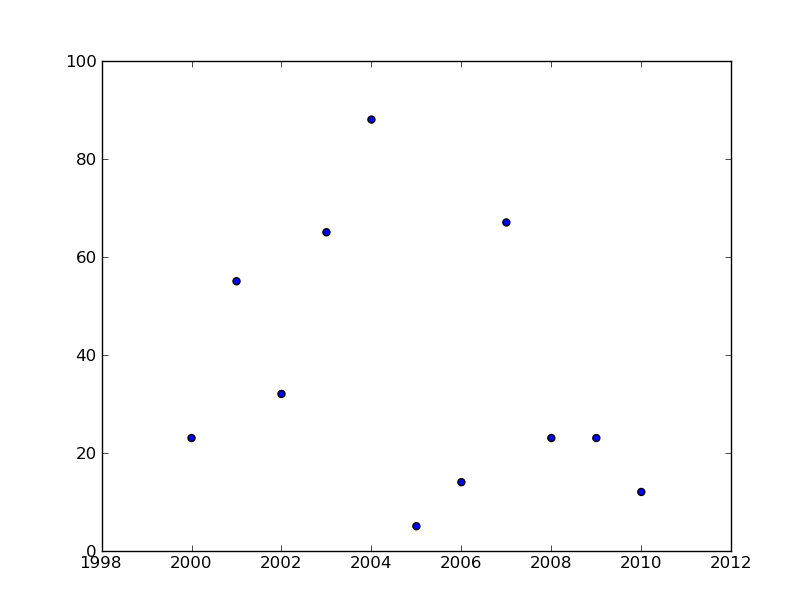
\includegraphics[scale=0.45]{../advanced_python/images/scatter.png}\\
\end{frame}

\begin{frame}[fragile]
  \frametitle{Pie Chart}
  \begin{lstlisting}
   In[]: pie(profit, labels=year)
  \end{lstlisting}
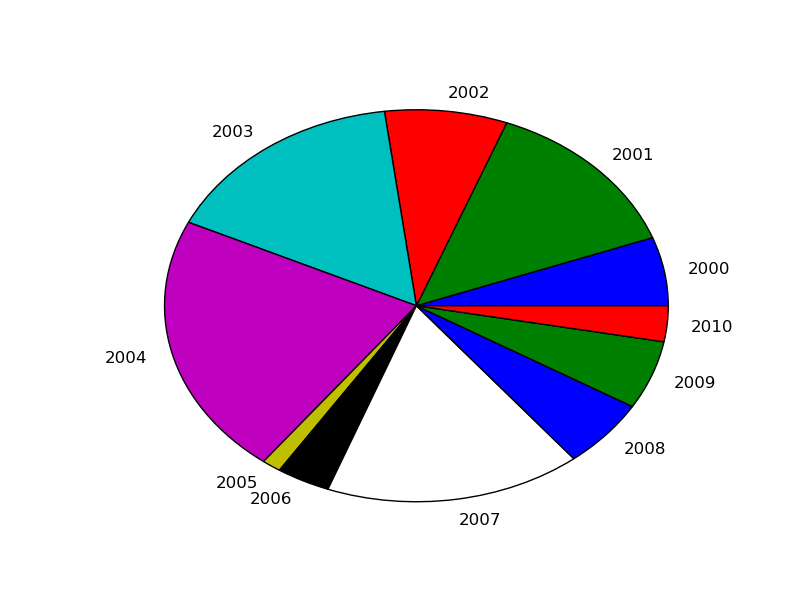
\includegraphics[scale=0.35]{../advanced_python/images/pie.png}\\
\end{frame}

\begin{frame}[fragile]
  \frametitle{Bar Chart}
  \begin{lstlisting}
   In[]: bar(year, profit)
  \end{lstlisting}
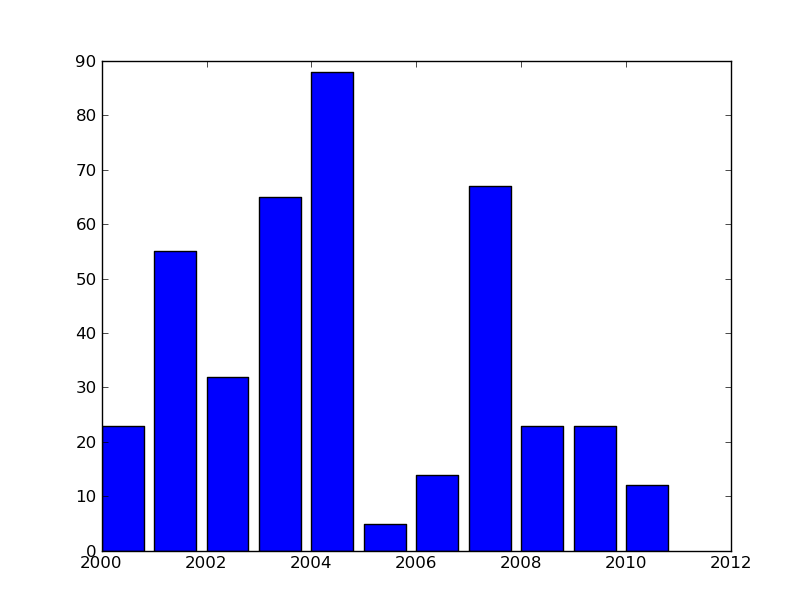
\includegraphics[scale=0.35]{../advanced_python/images/bar.png}\\
\end{frame}

\begin{frame}[fragile]
  \frametitle{Log-log plot}
  \begin{itemize}
  \item Plot a \texttt{log-log} chart of $y=5x^3$ for x from 1 to 20
  \end{itemize}
  \begin{lstlisting}
   In[]: x = linspace(1,20,100)
   In[]: y = 5*x**3

   In[]: loglog(x, y)
   In[]: plot(x, y)
  \end{lstlisting}
  \begin{itemize}
  \item Look at \url{http://matplotlib.sourceforge.net/contents.html}
    for more!
  \end{itemize}
\end{frame}

\begin{frame}
\frametitle{Log-log plot Plot}
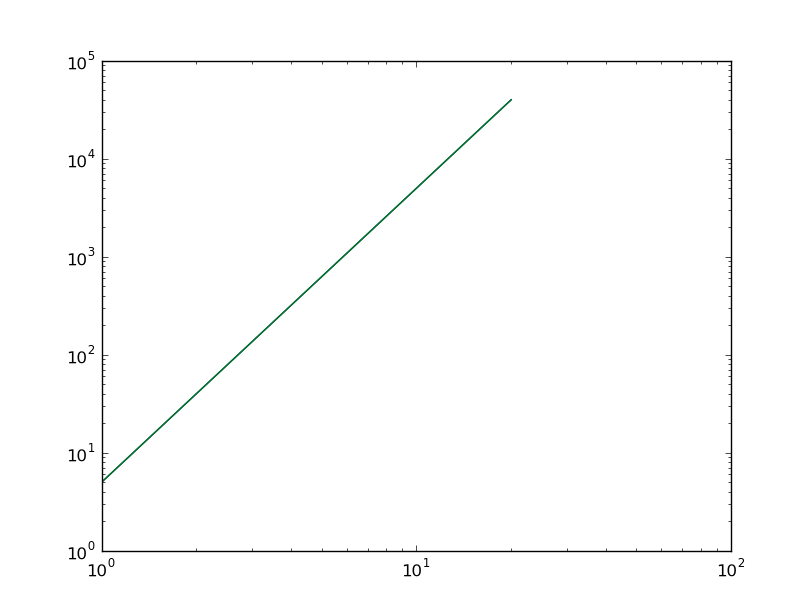
\includegraphics[scale=0.45]{../advanced_python/images/loglog.png}\\
\end{frame}


